\documentclass[twocolumn]{article}

\usepackage{amsmath}
\usepackage{caption}
\usepackage{graphicx}
\usepackage{float}

% Make table names in captions boldfaced
\captionsetup[table]{labelfont=bf}
\captionsetup[figure]{labelfont=bf}

\begin{document}
	
\title{Measuring the Speed of Light Using the Fizeau-Foucault Method}
\author{Jack Nelson, Raymond Chang, Robert Gregory}
\date{October 2016}

 % hacky trick to get a one-column abstract in a two-column article
\maketitle
\begin{abstract}
	Determining the value of fundamental constants of nature has been a basic function of physics since the founding of modern science.
	In this paper, we report our efforts to measure the speed of light in air to within ten percent of the accepted modern definition of 299,792 km/sec using a modernized version of the Foucault-Fizeau technique.
	Despite multiple calibrations and resets of the experimental setup, our best measurement of the speed of light was 145,000 km/sec [TODO add uncertainty], approximately a factor of two less than the accepted value.
	Because of our low random uncertainty, this would seem to indicate an unaccounted-for systematic error in our experiment.
	Measures were taken to quantify and eliminate possible sources of systematic error in the experiment, including quantifying backlash in the micrometer used to make laser deflection measurements.
\end{abstract}	
\section{Introduction}
	\label{sec:Intro}
	The paper is structured as follows:
	
	\S\ref{sec:Intro} provides an overview of the measurement of the speed of light, starting with a summary of historical attempts dating back to the 17th century.
	An overview of our particular technique of measurement is given, as well as a derivation of the equation used to calculate the speed of light from the quantities directly measured in our method.
	\S\ref{sec:Methods} describes the detailed experimental technique used to arrive at our measurement, as well as a discussion of potential sources of error, and ways we attempted to eliminate error, both random and systematic.
	\S\ref{sec:Results} presents the results of our experiment, including a full description of all calculations made, as well as our error analysis.
	\S\ref{sec:Conclusion} summarizes our experiment and findings.
		
	\subsection{Historical Background}
	
		The finite nature of light's speed has been questioned for centuries. 
		Most studies of the speed of light measure the time required for the light to travel a given distance. 
		Because of the apparent instantaneity of its travel in most human-scale settings, it wasn’t until scientific techniques and instruments matured in the late 17th and early 18th centuries that the nature of the speed of light could truly be investigated. 
		
		In 1638, the famed Renaissance scientist Galileo Galilei theorized about the nature of light's travel in the form of a fictional conversation between three Italians, Salviati, Sagredo, and Simplicio, in his treatise \textit{Dialogues Concerning Two New Sciences}.\cite{galilei_dialogues_1638}
		In the treatise, the three Italians speculate whether the speed of light is finite or infinite, and conclude that, if it is finite, it must be of very great magnitude:
		
		\begin{quotation}
			\noindent
			\textit{\textbf{Sagredo}} \newline 
			\textit{But of what kind and how great must we consider this speed of light to be? 
			Is it instantaneous or momentary or does it like other motions require time? 
			Can we not decide this by experiment?}
			
			\noindent \newline
			\textit{\textbf{Simplicio}} \newline 
			\textit{Everyday experience shows that the propagation of light is instantaneous; for when we see a piece of artillery fired, at great distance, the flash reaches our eyes without lapse of time; but the sound reaches the ear only after a noticeable interval.}
			
			
			\noindent \newline
			\textit{\textbf{Salviati}} \newline
			\textit{The small conclusiveness of these and other similar observations once led me to
			devise a method by which one might accurately ascertain whether illumination, i.e., the propagation of light, is really instantaneous. The fact that the speed of sound is as high as it is, assures us that the motion of light cannot fail to be extraordinarily swift.}
		\end{quotation}
		
		Galileo, through Salviati, goes on to explain his design of an experiment to determine whether light's rate of travel is finite or instantaneous using two persons equipped with lanterns they can quickly cover and uncover separated by a distance of a few miles . 
		The idea, then, is that as soon as one person covers their lantern, the second person covers theirs. 
		If the first person sees any delay in the covering of the second's lantern, they can conclude that light's speed is finite. 
		On the other hand, if the first person detects no delay in the covering of the second's lantern, they can conclude that light is instantaneous.
		
		Of course, at the distances which Salviati proposes, the speed of light is much too large to be detected by human reflexes. 
		Salviati (Galileo) admits that his own attempt at the experiment was inconclusive:
		
		\begin{quotation}
			\noindent
			\textit{\textbf{Sagredo}} \newline
			\textit{This experiment strikes me as a clever and reliable invention. 
			But tell us what you conclude from the results.}
			
			\noindent \newline
			\textit{\textbf{Salviati}} \newline
			\textit{In fact I have tried the experiment only at a short distance, less than a mile, from
			which I have not been able to ascertain with certainty whether the appearance of the opposite light was instantaneous or not; but if not instantaneous it is extraordinarily rapid.}
		\end{quotation}
		
		Despite the flawed nature of Galileo's proposed experiment, he did identify the importance of having a long baseline distance to making an accurate measurement of the speed of light, if it was indeed finite.
		
		In the subsequent centuries following Galileo's inconclusive theorizing on light, several scientists made the case that light's travel was indeed finite. 
		In 1676, Danish astronomer Ole R\o{}mer used the timing of the eclipses of Jupiter's moon Io, appropriately discovered by Galileo in 1610, to demonstrate that light's speed was finite.\cite{romer_motion_1677}
		
		Astronomer Christian Huygens, R\o{}mer's contemporary, readily accepted R\o{}mer's findings, and used his observations to estimate the speed of light to be equivalent to 230,000 km/s, about 25\% less than the current accepted value.
		This marked the first numerical value for the speed of light given by a scientist.\cite{bobis_cassini_2008}
		
		A quarter century later in 1704, Isaac Newton wrote about R\o{}mer's findings in \textit{Opticks} and estimated it would take light ``seven or eight minutes" to travel from the Sun to the Earth.\cite{newton_opticks_1704} 
		In a 1729 letter to Edmond Halley published by the Royal Society of London, James Bradley reported the phenomenon of stellar aberration and estimated the Sun-Earth light travel time to be 8 minutes and 12 seconds, just seven seconds less than the modern accepted value of 8 minutes and 19 seconds.\cite{bradley_account_1729}
		
		\begin{table*}[!ht]
			\centering
			\begin{tabular}{c|llll}
				Year & Scientist(s)                 	& Method				& Value (km/sec)      & Percent Error \\ \hline
				1638 & Galileo Galilei              	& Covered Lanterns		& Inconclusive 		  & N/A           \\
				1676 & Ole R\o{}mer, Christian Huygens 	& Eclipse of Io			& 230,000 			  & 25\%          \\
				1729 & James Bradley					& Aberration of Light	& 301,000			  & 0.4\%		\\
				1849 & Hippolyte Fizeau             	& Toothed Wheel			& 315,000 			  & 5\%           \\
				1862 & Leon Foucault                	& Rotating Mirror		& 298,000 			  & 0.6\%         \\
				1878 & Albert Michelson             	& Rotating Mirror, 600m Baseline	& 299,910 & 0.04\%        \\
				1926 & Albert Michelson            		& Rotating Mirror, 35km Baseline		 & 299,798 & 0.001\%  \\
				1983 & Bureau International des Poids Mesures	& Standard Definition	& 299,792.458	& Exact   
			\end{tabular}
			\caption{\textbf{Measurements of the speed of light since the 17th century}}
			\label{tab:HistoricalMasurements}
		\end{table*}
		
		The first terrestrial scientific attempts to systematically measure the speed of light were made at first cooperatively, and then separately, by Hippolyte Fizeau and L\'{e}on Foucault starting around 1845.\cite{sanders_velocity_1965}
		Fizeau used a rotating toothed wheel to modulate a light source across a distance of 8km to a fixed mirror which reflected the light back to the cog wheel. 
		Fizeau increased the speed of the wheel until light from one notch in the wheel was blocked by the subsequent tooth on its return trip. With this technique, Fizeau calculated the speed of light to be 315,000km/sec, about 5\% higher than the modern value.\cite{sanders_velocity_1965}
		
		Charles Wheatstone in 1834 proposed using a rotating mirror rather than a cog wheel and measuring the returning light's displacement when reflected off the rotating mirror at high angular velocities. 
		This technique was more fully developed by Foucault starting in 1850, and in 1862 Foucault measured a value of 298,000km/sec using a baseline of only 20m.\cite{sanders_velocity_1965}
		
		Foucault's method was further refined and expanded by Albert Abraham Michelson in 1878 using a baseline of 600m, obtaining a result of 299,910km/sec.\cite{michelson_experimental_1878}
		Nearly fifty years later in 1926, Michelson attempted a more accurate measurement, this time using a precisely-measured baseline of 35km between Mount Wilson and Mount San Antonio near Pasadena, California.
		The refined experiment measured a value of 299,798$\pm$4 km/sec, which is within 0.001\% error of the modern value of 299,792 km/s.\cite{michelson_measurement_1927}
		
		Table \ref{tab:HistoricalMasurements} summarizes the historical measurements of the speed of light since the 17th century up to the modern standard definition by the Bureau International des Poids et Mesures in 1983.\cite{_bipm_1984}
		
		
	\subsection{Theory of Experiment}
		Our experimental technique is heavily based on the direct-measurement technique Fizeau and Foucault pioneered in the mid-19th century.
		The central apparatus of the experiment is a two-sided variable-speed rotating mirror powered by a DC electric motor.
		A red laser is focused onto the mirror while it rotates at angular speeds of up to 1,500Hz.
		A slightly concave fixed mirror is located approximately 6m away at angle $\theta$ relative to the incident laser path such that as the rotating mirror sweeps through angle $\theta$, it reflects laser light onto the fixed mirror.
		The concave fixed mirror then reflects the laser light and focuses it back onto the rotating mirror.
		
		\begin{figure}[!ht]
			\centering
			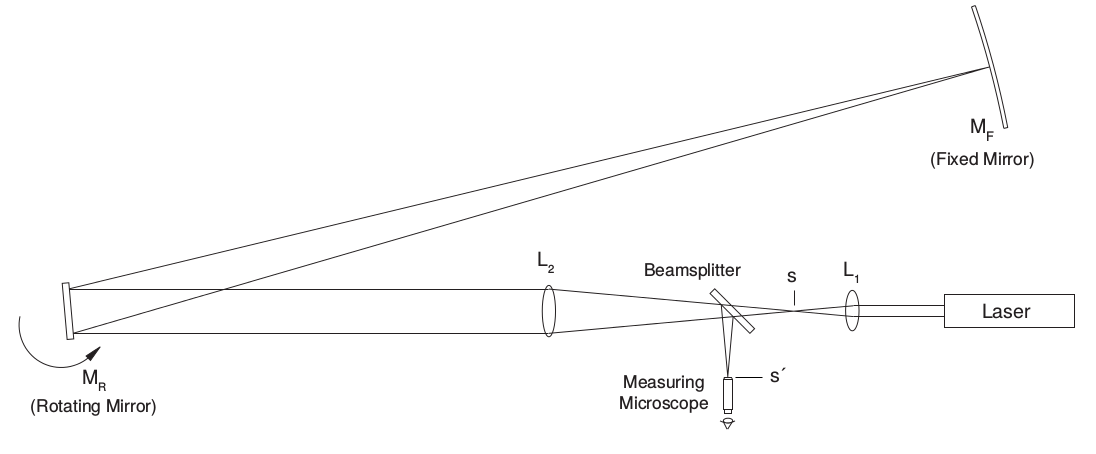
\includegraphics[width=0.49\textwidth]{Images/FoucaultMethodDiagram.png}
			\caption{\textbf{Configuration of a Fizeau-Foucault method of measuring the speed of light using a rotating mirror. Figure 1 of \cite{lee_instruction_????}. \copyright PASCO Scientific.}}
			\label{fig:FoucaultDiagram}
		\end{figure}
		
		If the speed of light were infinite and the travel time between the rotating and fixed mirrors instantaneous, the mirror would not rotate during the light's travel between the mirrors, and so the light would be reflected back towards the laser source at exactly the same angle it had entered.
		
		However, if the speed of light is finite, there should be a time-of-flight delay as the light travels from the rotating mirror to the fixed mirror and back.
		During this time, the rotating mirror should rotate an angular distance $\theta_s$, such that the angle of incidence of the light as it returns is slightly different from the angle of incidence of when it was initially reflected.
		This results in the returning light being slightly deflected from its original path incident to the rotating mirror.
		
		If we place a half-silvered beam splitter in between the laser source and the rotating mirror such that light from the rotating mirror is partially reflected into a microscope, we can measure the minute deflection of the laser light due to the rotating mirror's motion during the light's time-of-flight delay.
		
		The experimental configuration described above is shown in Figure \ref{fig:FoucaultDiagram}.
		
		\subsection{Derivation of the Speed of Light Equation from Experimental Measurements}
		
\section{Methods and Procedures}
	\label{sec:Methods}
	\subsection{Method Description}
	\subsection{Derivation of the Speed of Light Equation}

\section{Results}
	\label{sec:Results}


	\subsection{Data}
		% raw deflection measurements
		\begin{table*}[] 
			
			\centering
			
			\begin{tabular}{c c c c c}
				\hline
				Trial ID & \begin{tabular}[c]{@{}c@{}}CW Measurement \\ (mm) ($\pm0.01$)\end{tabular} & \begin{tabular}[c]{@{}c@{}}CW Speed \\ (rev/s) ($\pm5$)\end{tabular} & \begin{tabular}[c]{@{}c@{}}CCW Measurement \\ (mm) ($\pm0.01$)\end{tabular} & \begin{tabular}[c]{@{}c@{}}CCW Speed \\ (rev/s) ($\pm5$)\end{tabular} \\ \hline
				11       & 10.17                                                          & 1503                                                        & 9.27                                                            & -1460                                                        \\
				12       & 10.19                                                          & 1505                                                        & 9.27                                                            & -1464                                                        \\
				13       & 10.18                                                          & 1510                                                        & 9.28                                                            & -1461                                                        \\ \hline
				21       & 10.16                                                          & 1506                                                        & 9.28                                                            & -1462                                                        \\
				22       & 10.18                                                          & 1503                                                        & 9.33                                                            & -1463                                                        \\
				23       & 10.22                                                          & 1507                                                        & 9.36                                                            & -1460                                                        \\ \hline
				31       & 12.00                                                          & 1508                                                        & 11.12                                                           & -1465                                                        \\
				32       & 12.00                                                          & 1505                                                        & 11.08                                                           & -1456                                                        \\
				33       & 12.00                                                          & 1507                                                        & 11.12                                                           & -1468                                                        \\
				34       & 12.10                                                          & 1510                                                        & 11.12                                                           & -1466  \\ \hline                                                     
			\end{tabular}
			\caption{\textbf{Laser deflection data taken during three separate sessions. Positive rotation speeds correspond to clockwise rotation of the rotating mirror, and negative speeds correspond to counterclockwise speeds.}}
			\label{tab:rawmeasure}
		\end{table*}
		
		
		
	Three sets of data were taken spread across three measurement sessions on different dates. 
	The first two measurement sessions used the same experimental setup on different days. 
	Session three occurred after the experiment was broken down and rebuilt so as to try and exonerate the experimental setup as a source of error in the measurements. 
	As a result, the first two sets of data can be analyzed together, while the third set of data must be analyzed separately at first, since the process of rebuilding the experimental setup introduced systematic differences to the measurements made during the third session. 
	Since the calculated speed of light value is dependent on relative measurements and not absolute measurements, this systematic difference between the first two sets of data and the third will be shown to be negligible in the overall calculation of the speed of light.
	
	Table \ref{tab:rawmeasure} shows the measurements taken in each of the three sessions.
	The data is indexed by a trial ID. 
	The session each measurement belongs to is indicated by the leading digit of the Trial ID. 
	For example, measurement 23 is the third measurement taken during the second set of data.
	
	For the first two sessions, data was only taken for the $\pm$1500 rev/s rotating mirror speeds. 
	In the third set, additional measurements were made at mirror speeds $\pm$1000 rev/s in order to characterize backlash in the micrometer knob.
	
	Other values necessary for the calculation of the speed of light included the distance A between $L_1$ and $L_2$, the distance $B$ between $L_2$ and the rotating mirror, and the baseline distance $D$ between the rotating mirror and the fixed mirror. Measurements of each of these distances were taken for each set and are reported in Table \ref{tab:distances}.
		
	% distance measurement data
	\begin{table}[]
		\centering
		\begin{tabular}{c c c c }
			\hline
			& \begin{tabular}[c]{@{}c@{}}A(m)\\ ($\pm$0.005m)\end{tabular} & \begin{tabular}[c]{@{}c@{}}B(m)\\ ($\pm$0.005m)\end{tabular} & \begin{tabular}[c]{@{}c@{}}D (m)\\ ($\pm$0.01m)\end{tabular} \\ \hline
			Set 1 & 0.26                                                       & 0.481                                                      & 6.65                                                       \\
			Set 2 & 0.26                                                       & 0.481                                                      & 6.65                                                       \\
			Set 3 & 0.326                                                      & 0.45                                                       & 6.63      \\ \hline                                                
		\end{tabular}
		\caption{\textbf{Measurements of the lengths $A$, $B$, and $D$.}}
		\label{tab:distances}
	\end{table}	
	
	
	\subsection{Calculations}
	The equation for calculating the speed of light is dependent on the deflection difference between measurements at the maximum rotation speeds clockwise and counter-clockwise. 
	Table \ref{tab:deflection} shows the deflections for each measurement in mm.
	
	% deflection data
	\begin{table}[t]
		\centering
		\begin{tabular}{c c}
			\hline
			Trial ID & \begin{tabular}[c]{@{}c@{}}Deflection \\ (mm)\end{tabular}  \\ \hline
			11       & 0.90       \\
			12       & 0.92       \\
			13       & 0.90       \\
			21       & 0.88       \\
			22       & 0.85       \\
			23       & 0.86       \\
			31       & 0.88       \\
			32       & 0.92       \\
			33       & 0.88       \\
			34       & 0.98       \\                                              
		\end{tabular}%
		\caption{\textbf{Deflection measurements of the laser between the maximum rotation speeds in the clockwise and counterclockwise directions, in mm and m.}}
		\label{tab:deflection}
	\end{table}
	
	Comparing the measurements in sets 1 and 2 to those in set 3, we can see that the absolute value of these measurements are different, yet the relative deflections are still roughly the same. 
	This indicates that our experimental setup was consistent and did not affect the outcome of the measurements. 
	This will be further supported in the section on error analysis.
	
	To calculate a value for the speed of light, each set of measurements was averaged with respect to mirror rotation speed and direction. 
	The average measurement values for each set are shown in table \ref{tab:meanvalues}. 
	The mean deflection for each set was calculated from the difference of the mean measurements at +1500 rev/s and -1500 rev/s.
	
	% mean measurements data
	\begin{table*}[t]
		\centering
		\begin{tabular}{c c c c}
			\hline
		    Data Set	& \begin{tabular}[c]{@{}c@{}}Measurement Mean, CW\\ (mm)\end{tabular} & \begin{tabular}[c]{@{}c@{}}Measurement Mean, CCW\\ (mm)\end{tabular} & \begin{tabular}[c]{@{}c@{}}Mean Deflection\\ (mm)\end{tabular} \\ \hline
			Set 1 & 10.18                                                               & 9.27                                                                 & 0.91                  \\
			Set 2 & 10.18                                                               & 9.32                                                                 & 0.86                                                   \\
			Set 3 & 12.02                                                               & 11.11                                                                & 0.92                                        \\       
		\end{tabular}
		\caption{\textbf{Mean measurements for each set of data averaged with respect to mirror rotation speed and direction.}}
		\label{tab:meanvalues}
	\end{table*}
	
	The rotation frequencies for each measurement were recorded as well and averaged for each set. 
	The total rotation frequency $f_{CW}+f_{CCW}$ is just the sum of the mean rotation frequencies for each set, and is used in the calculation of the speed of light. 
	These values are reported in table \ref{tab:averagerotf}.
	
	% average rotation speed data
	\begin{table*}[t]
		\centering
		\begin{tabular}{c c c c}
			\hline
			 Data Set & \begin{tabular}[c]{@{}l@{}}Mean CW Rotation Speed \\ (Rev/s)($\pm$5)\end{tabular} & \begin{tabular}[c]{@{}l@{}}Mean CCW Rotation Speed \\ (Rev/s)($\pm$5)\end{tabular} & \begin{tabular}[c]{@{}l@{}}Mean Deflection Frequency \\ (Rev/s)($\pm$10)\end{tabular} \\ \hline
			Set 1 & 1506                                                                            & -1461                                                                             & 2967                                                                               \\
			Set 2 & 1505                                                                            & -1462                                                                             & 2967                                                                               \\
			Set 3 & 1508                                                                            & -1464                                                                             & 2971  \\                                                                      
		\end{tabular}
		\caption{\textbf{Mean measurement rotation speeds for each set of data.}}
		\label{tab:averagerotf}
	\end{table*}
	
	The speed of light $c$ for each set was calculated using the mean deflections $s'_{cw}-s'_{ccw}$, the rotation speed difference $f_{cw} + f_{ccw}$, the distances $A$, $B$, and $D$, and the equation described in Methods and Procedures and restated in below as Equation \ref{eq:speedoflight_calcs}.
	
	\begin{equation} \label{eq:speedoflight_calcs}
	c = \frac{ 8\pi AD^2 (f_{cw} + f_{ccw})}
			 { (D + B) (s'_{cw} - s'_{ccw})}
	\end{equation}
	
	The calculated speed of light $c$ for each set of data is shown in Table \ref{tab:cvals}.
	
	% speed of light
	\begin{table*}[!ht]
		\centering
		\begin{tabular}{c c c c} \hline
			Data Set  & \begin{tabular}[c]{@{}c@{}}$c$ \\ ($m/s$)\end{tabular} & \begin{tabular}[c]{@{}c@{}}Random Uncertainty \\ ($\pm m/s$)\end{tabular} & \begin{tabular}[c]{@{}c@{}}Systematic Uncertainty \\ ($\pm m/s$)\end{tabular} \\ \hline
			Set 1 & $1.33*10^{8}$                                           & TODO	& TODO                                                             \\
			Set 2 & $1.39*10^8$                                           & TODO	& TODO                                                             \\
			Set 3 & $1.65*10^8$                                           & TODO	& TODO                       \\                                   
		\end{tabular}
		\caption{\textbf{Calculated values of the speed of light}}
		\label{tab:cvals}
	\end{table*}
	
	\subsection{Error Analysis} \label{subsec:error}
	Each set of data was separately analyzed for random and systematic error.
	For each data set, the standard deviation of each of each measurement at each frequency was calculated, then added in quadrature to arrive at a standard deviation of uncertainty in the deflection value.
	 
	\subsection{Discussion}


\section{Conclusion}
	\label{sec:Conclusion}

\bibliographystyle{siam}
\bibliography{SpeedofLight}

\end{document}
